\documentclass{article}
\usepackage{graphicx} 
\usepackage{float}
\usepackage{booktabs}
\usepackage{array}
\usepackage{arydshln}
\usepackage{siunitx}
\usepackage{hyperref}
\usepackage{cancel}
\usepackage{changepage}
\usepackage{placeins}
\usepackage{enumitem}


\usepackage{tabularx}
\usepackage{amsmath, amssymb, amscd, MnSymbol, mathrsfs}
\usepackage{cellspace}
\usepackage{tikz}
\usetikzlibrary{calc, patterns, angles, quotes, decorations.markings, decorations.pathmorphing, hobby}
\usepackage{xfrac}

\usepackage{chemfig}
\usepackage{caption}
\usepackage{tcolorbox}
\usepackage{bm}
\usepackage{pdfpages}
\usepackage{empheq}
\usepackage{pgfplots}
\pgfplotsset{compat=1.18}
\usepackage[oldvoltagedirection]{circuitikz}
\usepackage{microtype}
\usepackage{tikz-3dplot}
\usepackage{bibref}
\usepackage{textcomp}
% Custom commands
\newcommand{\vect}[1]{\boldsymbol{\mathbf{#1}}}
\newcolumntype{C}{>{\centering\arraybackslash}X}
\newcolumntype{M}[1]{>{\centering\arraybackslash}m{#1}}

\usetikzlibrary{external}
\tikzexternalize[prefix=figures/]

\newcommand\myfrac[2]{\sfrac{#1\mkern-1.2mu}{#2}}
\usepackage{xcolor}

% Define custom colors
\definecolor{darkblue}{rgb}{0.1,0.1,0.5} % A dark blue shade
\definecolor{formalshade}{rgb}{0.95,0.95,1} % A light blue shade for the background

% For the adjustwidth environment
\PassOptionsToPackage{strict}{changepage}
\usepackage{changepage}

% For formal definitions
\usepackage{framed}

\newcommand{\formalsource}{} % Initialize an empty macro to store the source text

\newenvironment{formal}[1][]{% Start of the environment
    \renewcommand{\formalsource}{#1}% Store the optional argument
    \def\FrameCommand{%
        \hspace{1pt}%
        {\color{darkblue}\vrule width 2pt}%
        {\color{formalshade}\vrule width 4pt}%
        \colorbox{formalshade}%
    }%
    \MakeFramed{\advance\hsize-\width\FrameRestore}%
    \noindent\hspace{-4.55pt}% Disable indenting the first paragraph
    \begin{adjustwidth}{}{7pt}%
        \vspace{2pt}%
    }%
    {%
        \vspace{2pt}%
        \ifx\formalsource\empty % Check if the source is empty
        \else
        \hfill{\footnotesize\textit{Source: \formalsource}}% Align source to the bottom-right
        \fi
    \end{adjustwidth}\endMakeFramed%
}


% Custom itemize list with images for positive and negative items
\newlist{gitemize}{itemize}{1} % Just one level for the list
\setlist[gitemize,1]{
    leftmargin=2.8em, % Adjust the margin for the list
    labelsep=1em % Control the space between the label and the list item
}

% Define checkmark and cross symbols for positive and negative items
\newcommand{\checkitem}{\raisebox{-0.25\height}{\includegraphics[width=0.4cm]{checkmark.png}}}
\newcommand{\crossitem}{\raisebox{-0.25\height}{\includegraphics[width=0.4cm]{cross.png}}}


\usepackage[margin=1in, left=0.8in, right=0.8in, includeheadfoot]{geometry}
\usepackage{fancyhdr}
\usepackage{graphicx}
\usepackage{tabularray}

\pagestyle{fancy}
\fancyhf{}


\renewcommand{\headrulewidth}{0.4pt}
\renewcommand{\footrulewidth}{0.4pt}

\fancyhead[L]{
\includegraphics[height=1.2cm]{images/Kingston_University_London_logo_200-tablet.png}}
\fancyhead[R]{EG4019 - ME - Engineering Mechanics and Materials}
\fancyfoot[C]{Department of Mechanical Engineering}
\fancyfoot[R]{\thepage}

\geometry{top=0.5in,bottom=0.7in}
\usepackage{scalerel}

\setlength{\headheight}{30pt}
\setlength{\footskip}{20pt}


\usepackage[export]{adjustbox}
\usepackage{tocloft}
\renewcommand{\cfttoctitlefont}{}
\renewcommand{\contentsname}{}
\renewcommand{\cftsecleader}{\cftdotfill{\cftdotsep}}

\setlength{\cftbeforesecskip}{0.5em}


\usepackage{xurl}

\renewcommand{\theequation}{\text{Eq.}~\arabic{equation}}
%Refer to the equation as \eqref{equation}.
\usepackage{caption}  % This package allows captioning outside of a float
\begin{document}
        

    \vspace*{\fill}
    \begin{center}
        \textbf{\Huge Laboratory Report}\\[10pt]
        \LARGE \textbf{Tensile Test}
    \end{center}
    \vspace*{\fill}

    \Large    
    \begin{tabular}{@{}l l l@{}}
        \textbf{Submitted by:} & Sakariye Abiikar (Group Leader) & K2371673 \\
        & Sandeep Singh & K2314795 \\
        & Aland Floyd Noronha & K2423819 \\
        & Alan Roy & K2314478 \\
        & Judas Surname & K5671234 \\
    \end{tabular}
    
    \vspace*{\fill}
    
    \begin{tabular}{@{}l l@{}}
        \textbf{Key Dates:} & Date of practical: \\
        & Deadline: 31/12/2024 \\
        & Date of submission: \\
    \end{tabular}
    \vspace*{\fill}
    
    \large
    \newpage\noindent\vspace{2em}
    \begin{center}
        \LARGE \textbf{Contribution Table}\\[3em]
    \end{center}
    

    
    \begin{tblr}{
            colspec={Q[4cm]Q[4cm]Q[4cm]Q[3cm]},
            hlines,vlines,
            cells={valign=m,halign=c},
            rows={ht=4\baselineskip},
            row{1}={ht=1.5\baselineskip,font=\bfseries},
        }
        Student & Course & Contribution & Picture \\ 
        Sakariye Abiikar & Mechanical Engineering & Results, Theory, Recommendations & 
\includegraphics[width=2cm,valign=c]{images/profile.jpg} \\ 
        Andrew Surname & Aviation & Introduction & 
\includegraphics[width=2cm,valign=c]{images/profile.jpg} \\ 
        Lucas Surname & Astro & Results & 
\includegraphics[width=2cm,valign=c]{images/profile.jpg} \\ 
        James Surname & Mechanical Engineering & Discussion, References & 
\includegraphics[width=2cm,valign=c]{images/profile.jpg} \\ 
        Judas Surname & Civil Engineering & No Contribution & 
\includegraphics[width=2cm,valign=c]{images/profile.jpg} \\ 
    \end{tblr}
    
    \normalsize
    \newpage\noindent\vspace{1em}
    \begin{center}
        \LARGE \textbf{Table of Contents}\\[1.5em]
    \end{center}
    \tableofcontents
    \thispagestyle{fancy}


    \large\newpage\vspace*{-20pt}

    \section{Abstract}
    \vspace*{1em}
    This study investigated the effects of two thermal treatments on the mechanical properties of HE30/BS1476 aluminium alloy, initially characterized by a hardness of 120 HV5, an elastic modulus of 6 GPa, and an ultimate tensile strength of 500 MPa. The alloy underwent two heat treatments: first, heating for 90 minutes at 520\textdegree C, followed by an additional 40 minutes at 184\textdegree C in open air. Three distinct alloy variations were produced as a result of these treatments. The aim of the research was to quantify changes in hardness, modulus of elasticity, yield strength, ultimate tensile strength (UTS), and percentage elongation. Hardness was measured using a Zwick Roell ZHU hardness testing machine with a 5 kg load (HV5) (See Appendix A), and properties such as stress and strain were derived from data obtained using a Zwick Roell 2050 tensile testing machine.
%   {Needs small info on results and reflection/conclusion (to be added at a later date)}
   
    
    \newpage\vspace*{-20pt}
    \section{Introduction}

    In engineering, the selection and optimization of materials directly impact the performance of a design application, especially in aerospace, automotive, and construction industries.\\[8pt] 
    Aluminium alloys have a good strength-to-weight ratio and corrosion resistance; therefore, they are very important in such sectors, though mostly in applications requiring specific mechanical improvements through controlled processes. \\[8pt] 
    Research by metallurgists such as Sorby and Sauveur demonstrated that \textbf{heat treatment} significantly improves the properties of alloys. By changing the alloy's microstructure, these heat treatments improve its tensile strength, hardness, and elasticity. Various heat treatment techniques, including quenching and solution heat treatment, are designed to accomplish particular mechanical qualities based on the alloy's intended use.\\[8pt] 
    The \textbf{aging process} is a critical aspect of heat treatment, fundamental to precipitation hardening, as highlighted by metallurgists like William Hume-Rothery.It enhances the material's properties by promoting the formation of fine precipitates, which obstruct dislocation movement, thereby increasing the alloy's strength and hardness, it is thoroughly regulated in terms of temperature and time in order to maximise the distribution of these precipitates.\\[8pt] 
    For example, one study applying these strategies involved a solution heat treatment of Al 6082 alloy for 8 hours, resulting in an increase in hardness from 65 BHN to 102 BHN. Additionally, its tensile strength rose from 154 MPa to 280 MPa after 6 hours of aging at 205°C and 495°C (Singh, R., Singh, P., \& Das, 2023). \\[8pt] 
    These microstructural enhancements allow aluminium alloys such as HE30 to be used in very demanding applications in the aerospace and automotive industries.\\[8pt] 
    This research work investigates the response of HE30 aluminium alloy to thermal treatments by observing the changes in mechanical properties.  
            
    \newpage\vspace*{-20pt}
\section{Method}
This laboratory research primarily focused on the evaluation of the mechanical properties of our alloy samples, specifically key metrics such as yield strength, ultimate tensile strength (UTS), modulus of elasticity, hardness, and percentage elongation. These properties are essential for understanding the material's behavior under stress and are typically used to assess the material’s suitability for different engineering applications.\\[8pt]
The methodology applied in this research was designed around an \textbf{integrated testing strategy}—an approach that aims to maximize the amount of data obtained from each step while ensuring the highest level of accuracy and efficiency. This is often referred to as \textbf{data-driven experimentation} or \textbf{multivariate analysis}, where multiple factors are measured simultaneously to extract a fuller picture of material properties with minimal effort.\\[8pt]
The \textbf{goal-oriented design} of the methodology is based on the principle of reducing experimental redundancy while maximizing the information gathered. For example, a single tensile test can yield data on multiple properties (e.g., UTS, yield strength, modulus of elasticity) with the help of carefully selected test parameters and data analysis methods.\\[8pt]
This principle is at the heart of experimental optimization, often involving methods like \textbf{response surface methodology (RSM)} or \textbf{factorial design}, which help streamline the testing process by systematically varying and analyzing input parameters to identify the most efficient experimental conditions.\\[8pt]
By focusing on a minimal set of tests that can provide insights into multiple properties, this methodology ensures that each procedure is maximally informative, thus minimizing resource usage and reducing the chances of error.\\[8pt]
Our approach was characterized by the following key components:
\begin{enumerate}[itemsep=-0.5mm]
    \item {Dimensional Analysis}
    \item {Hardness Testing}
    \item {Tensile Testing} 
    \item {Data analysis}
\end{enumerate}
Note that \textbf{Sample Preparation} is distinct from the testing process and is not considered part of the testing itself.\\[1em]
This comprehensive and interconnected approach underscores the efficiency of our laboratory testing methodology. By designing experiments that yield multiple insights from each procedure, we were able to conduct a thorough analysis of the alloy's mechanical properties while minimizing resource usage and potential sources of error. This method not only ensures the accuracy and reliability of our results but also provides a rich dataset for in-depth analysis and interpretation of the alloy's performance characteristics.
\newpage

\section{Experimental Procedures}
The alloys used in this study are based on the HE30 (BS 1476) aluminium alloy. BS 1476, officially titled \textit{"BS 1476:1955 - Wrought Aluminium and Aluminium Alloys for General Engineering Purposes. Bars, Rods, and Sections,"} was introduced on December 22, 1955, and underwent several revisions reflecting advancements in materials science and engineering practices. The standard’s last revision occurred in 1987, and it remained active—with amendments—until its withdrawal on June 21, 2022.\\[1em]
While it is known that BS 1476 is no longer an operational standard, there is no publicly available evidence that it was directly replaced by a specific successor, such as those often published under European Norms (EN).\\[1em] 
Although the exact BS 1476 standards for HE30 are hard to come by, the composition and properties of the \textbf{6082 aluminium} alloy are often used as a contemporary substitute for HE30 in engineering processes.
\subsection{Description}
Key details are as follows:
\begin{formal}[Truventor, 27/03/2019]
Aluminium HE 30 alloy a.k.a AL 6082 is a medium strength alloy with excellent corrosion resistance. It
has the highest strength of 6000 (6XXX) series alloys. It is also known as a structural alloy. In block,
plate, or bar form, AL HE 30 alloy is most commonly used in machining.\\[1em]
Although it is a relatively new alloy, due to its higher strength, AL HE 30 has replaced AL 6061 in many
applications. The addition of a large amount of manganese controls the grain structure which in turn
results in a stronger alloy.\\[1em]
\textbf{Characteristics:}
\begin{itemize}
    \item High strength-to-weight ratio makes it ideal for lightweight structures.
    \item Most versatile and highest strength alloy in the 6000 series Aluminum.
    \item Good machinability compared to metals like Stainless Steel (SS) and Mild Steel (MS).
    \item Lightweight and corrosion-resistant components.
    \item Alternative to plastics in high-stress applications.
    \item Lower fatigue strength and elastic strength compared to steels.
\end{itemize}
\textbf{Applications:}
\begin{itemize}
    \item Automotive components.
    \item Electronic applications.
    \item Aerospace components.
    \item Trusses, frames, and beams.
\end{itemize}
\vspace{-8pt}
\end{formal}\noindent
While it is common practice to treat HE30 as equivalent to Aluminium Alloy 6082, minor differences in composition and performance may exist between HE30 under BS 1476 and 6082. For more precise specifications of HE30 under BS 1476, consulting the British Standards Institution (BSI) may provide further clarity, especially since the standard was withdrawn in 2022.\\[1em]
For the purposes of this work, HE30 will be treated as equivalent to 6082, which serves as the basis for further analysis of its properties and related topics, i hope you can understand.
\subsection{Composition}
\centering
\begin{minipage}{0.4\textwidth}
    \centering
    \renewcommand{\arraystretch}{1.4}
    \begin{tabular}{|>{\normalsize\bfseries}l|>{\normalsize}c|}
        \hline
        \large\textbf{Chemical Element} & \large\textbf{\% Present} \\ \hline
        Aluminium (Al)            & Remainder           \\ \hline
        Silicon (Si)              & 0.7-1.3\%           \\ \hline
        Magnesium (Mg)            & 0.6-1.2\%           \\ \hline
        Manganese (Mn)            & 0.4-1.0\%           \\ \hline
        Iron (Fe)                 & 0.5\% max           \\ \hline
        Copper (Cu)               & 0.1\% max           \\ \hline
        Zinc (Zn)                 & 0.2\% max           \\ \hline
        Chromium (Cr)             & 0.25\% max          \\ \hline
        Titanium (Ti)             & 0.1\% max           \\ \hline
        Residuals                 & 0.15\% max          \\ \hline
    \end{tabular}
    \captionof{table}{Chemical Composition of 6082 (HE-30) Alloy (Truventor, 2019)}
    \label{tab:composition_6082}
    \vspace{1em}
    \begin{tabular}{|>{\normalsize\bfseries}l|>{\normalsize}c|}
        \hline
        \large\textbf{Chemical Element} & \large\textbf{\% Present} \\ \hline
        Aluminium (Al)            & Remainder           \\ \hline
        Copper (Cu)               & 0.1\% max           \\ \hline
        Magnesium (Mg)            & 0.4 - 1.5\%         \\ \hline
        Silicon (Si)              & 0.6 - 1.3\%         \\ \hline
        Iron (Fe)                 & 0.6\% max           \\ \hline
        Manganese (Mn)            & 0.4 - 1.0\%         \\ \hline
        Zinc (Zn)                 & 0.1\% max           \\ \hline
        Chromium (Cr)             & 0.5\% max           \\ \hline
        Titanium (Ti)             & 0.2\% max           \\ \hline
    \end{tabular}
    \captionof{table}{Chemical Composition of HE30 according to Dr. Santiago's Data}
    \label{tab:composition_he30}
\end{minipage}
\hfill
\begin{minipage}{0.55\textwidth}
    The composition of HE30 (also known as 6082) generally follows the typical values for 6082 aluminium alloy, as shown in Table \ref{tab:composition_6082}.\\[1em]
    Once again, I stress that there may be minor differences in the composition of HE30, especially in accordance with the BS 1476 specifications.\\[1em] 
    The values listed here are provided for reference, but the exact composition of the HE30 alloy should be verified for accurate work in our lab, as it may not align with typical web standards.
    \vspace{1em}\hrule\vspace{1em}
    Although I do have actual information regarding the "Aluminium alloy HE30 BS1476" from Dr. Santiago shown in Table \ref{tab:composition_he30}, it is important to note that this source lacks proper documentation, and its credibility remains uncertain.\\[1em]
    This information contradicts much of the current research surrounding the HE30 BS1476, as i iterated that the standard has been withdrawn and has not been explicitly updated or replaced; it is still mainly unreferenced and not widely recognised in the contemporary literature, as such is why i adopted the 6082.\\[1em]
    Although there are slight differences between the two sources in terms of composition, I have chosen to adopt Dr. Santiago's version for the purpose of this work. This decision is based on the fact that the table he provided reflects the information he, as my instructor, has shared with me. While I acknowledge the discrepancies and the lack of clear sourcing in his data, I consider it appropriate to proceed with his version for expediency, particularly as it aligns with the guidance he has given in our coursework.
\end{minipage}\\

\raggedright

\subsection{Heat Treatments and Alloy Conditions}
Each sample was treated under different conditions to evaluate the effect of heat treatment on its mechanical properties. The samples were provided in the typical bone-shaped form for tensile testing. The heat treatment conditions are as follows:
\begin{itemize}[itemsep=-1mm]
    \item \textbf{AR (As Received)}: The sample was used without any heat treatment, in its initial state as supplied.
    
    \item \textbf{ST (Solution Treatment)}: The sample was heated at 520\textdegree C for 90 minutes to dissolve precipitates, improving ductility. The exact quenching method is unspecified.
    
    \item \textbf{PH (Precipitation Hardening)}: The sample was first heated at 520\textdegree C for 90 minutes, followed by aging at 184\textdegree C for 40 minutes to enhance strength and hardness.
\end{itemize}
These treatments were applied to assess how they influence the alloy's mechanical properties.



% Here is the guidline/rules for this subsection
% Experimental procedures describe the precise, step-by-step actions required to carry out an experiment—such as specific instructions like "do this" or "do that"—ensuring repeatability and accuracy in obtaining results. These procedures are intended to allow any individual to physically replicate the experiment.

%SAMPLES: 
% Description of the alloy, Composition, CSA (mention dimensions are measured by a calliper), Nomenclature, Heat treatments, Picture before testing, etc

% HARDNESS: 
% Testing machine (pics), Procedure (pics)

% TENSILE TEST: 
% Machine (pics), Procedure (pics)

%\begin{figure}[H]
%    {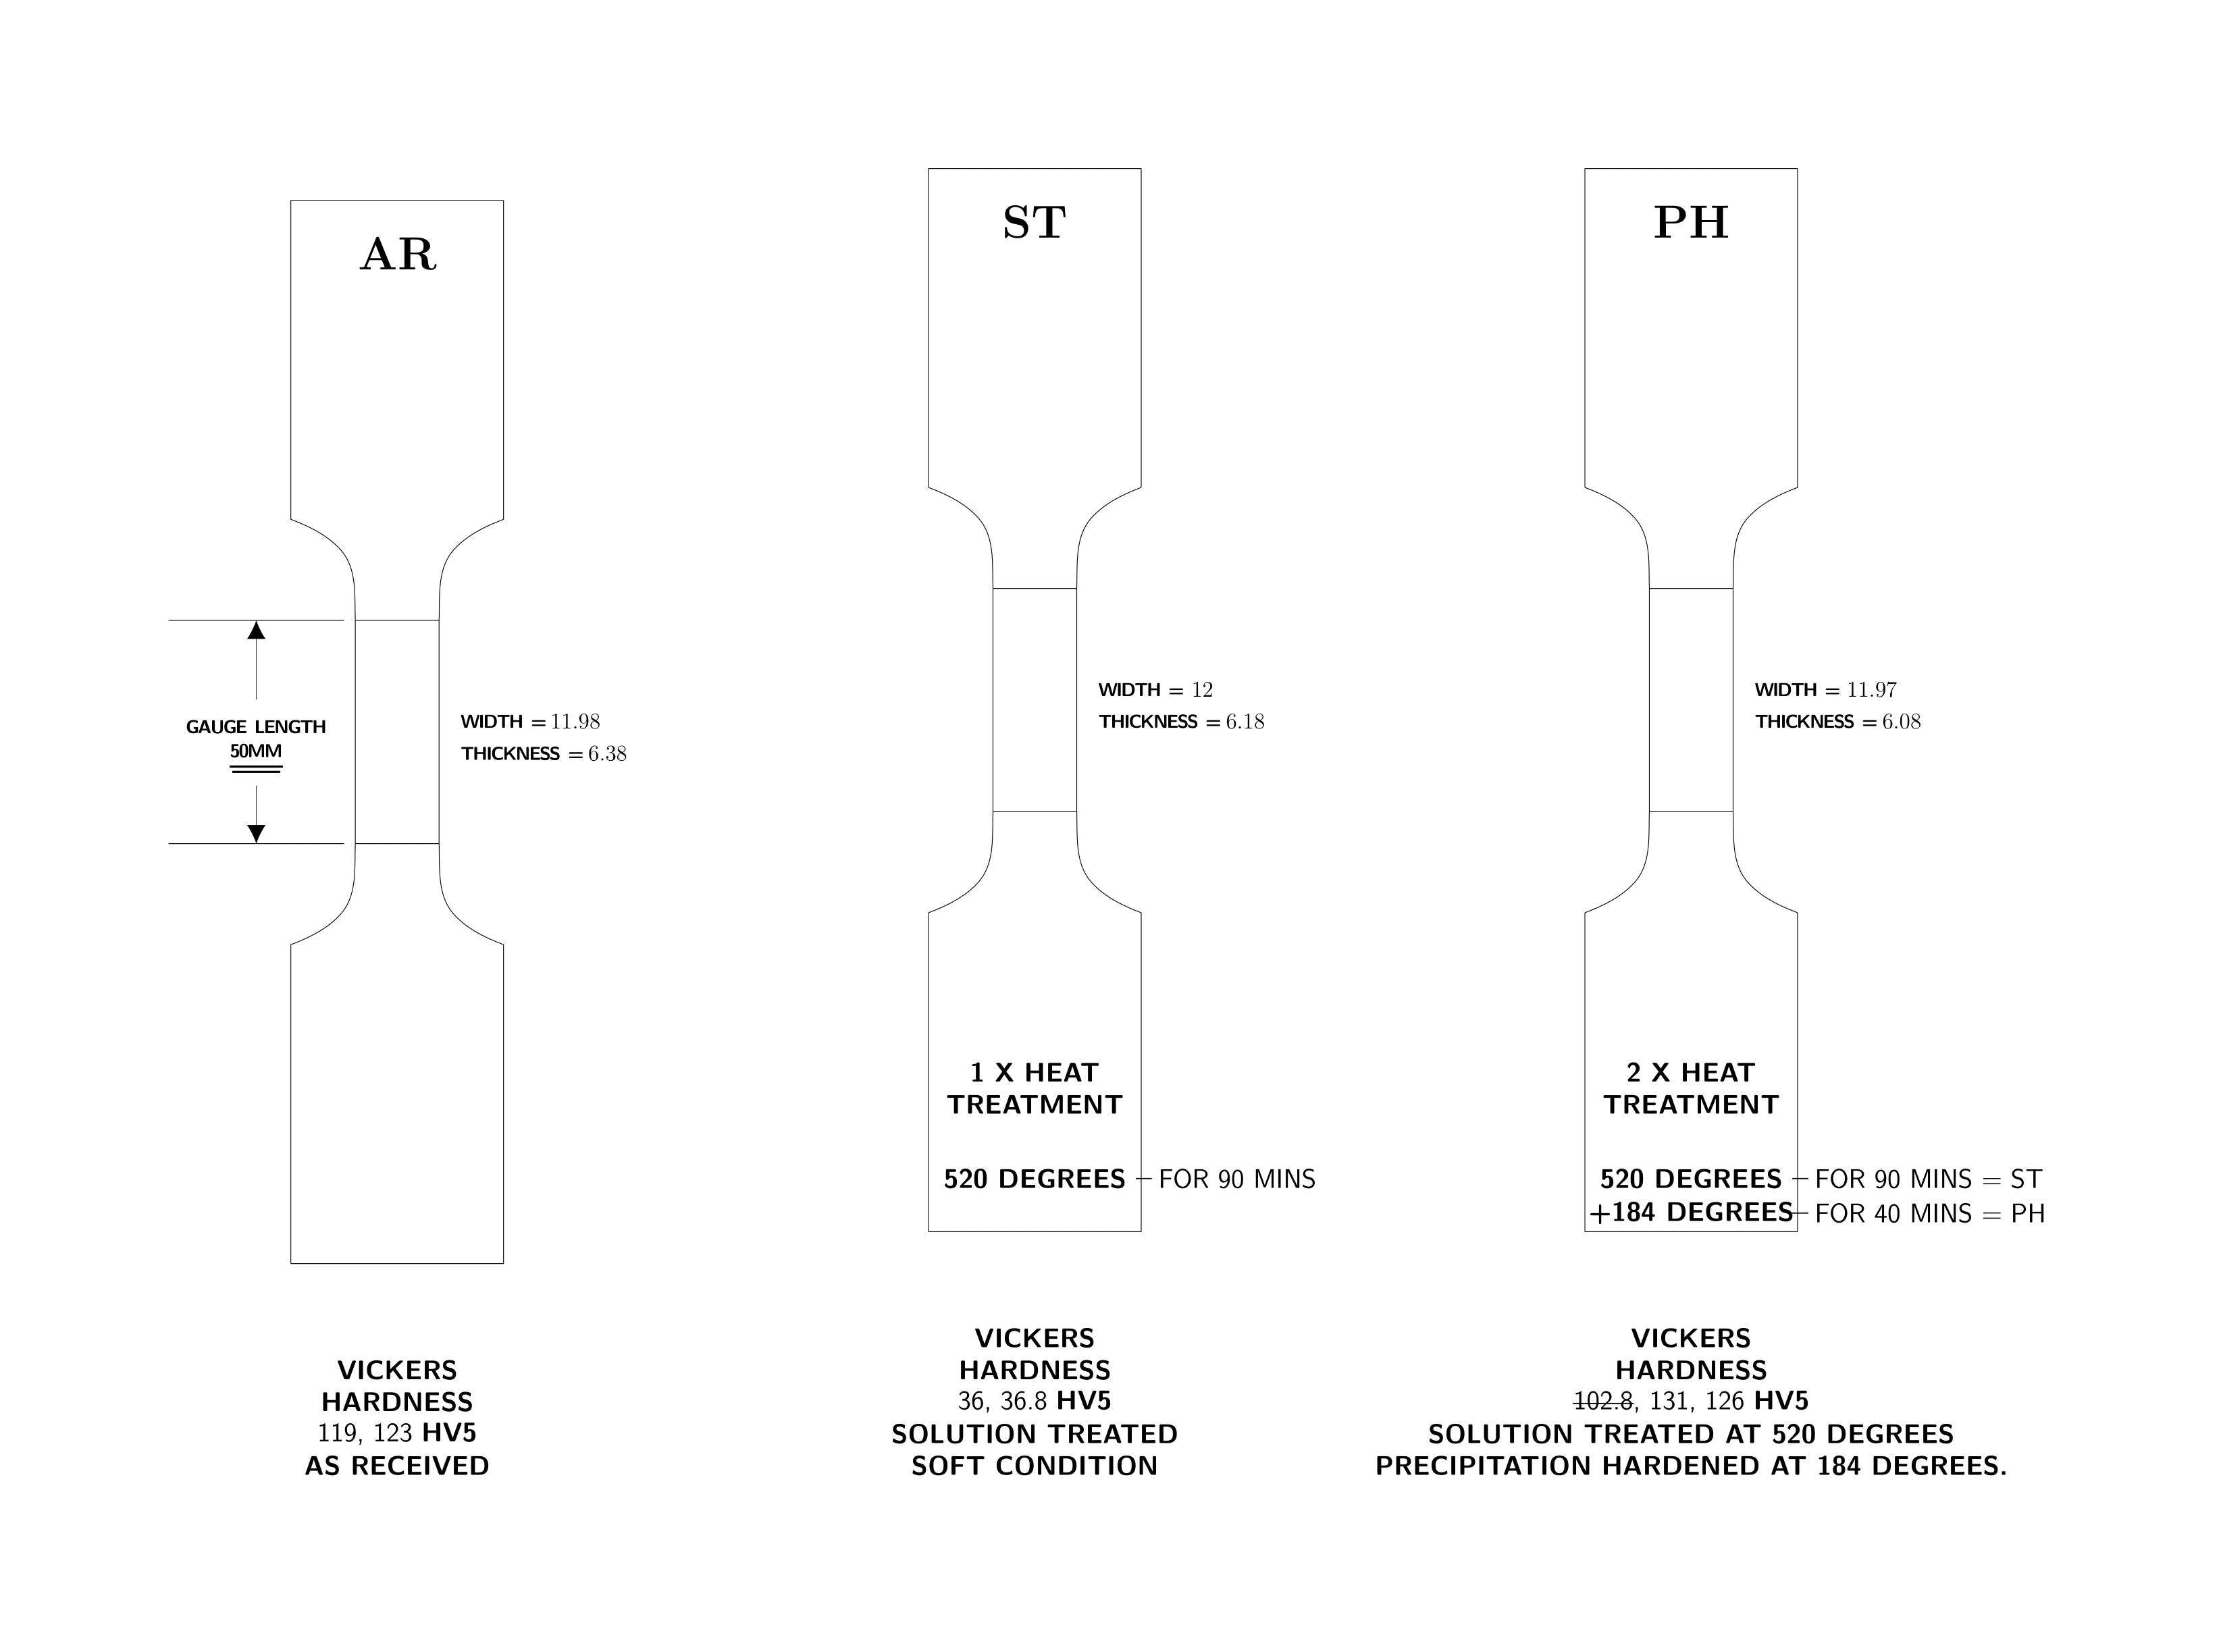
\includegraphics[width=\textwidth]{images/alloys.png}}
%    \caption{alloys}
%    \label{fig:alloys}
%\end{figure}
\subsection{Equipment List}
The following equipment was used during the experiments:
\begin{itemize}
    \item \textbf{Digital Caliper}
    \item \textbf{Vickers Hardness Testing Machine}
    \item \textbf{Zwick Roell 2050 Tensile Testing Machine}
    \item \textbf{Personal Protective Equipment (PPE)}
    \item \textbf{Camera/Smartphone}
    \item \textbf{Miscellaneous Equipment}
\end{itemize}
\subsection{Risk Assessment}
The experimental procedures involved several potential hazards. The identified risks, their levels, and mitigation strategies are outlined below:
\begin{table}[h!]
    \centering
    \begin{tblr}{
            width=\linewidth,
            colspec={Q[4cm]Q[4cm]Q[2cm,c,m]Q[5cm]},
            row{1} = {font=\bfseries,c,m},
            rows,columns = {valign=m},
            hlines, vlines
        }
        Hazard & Risk & Level of Risk & Control Measures \\
        Sharp edges of dogbone samples & Cuts or injuries while handling samples & Medium & Handle with care; use gloves when measuring and mounting samples. \\
        Tensile testing machine & Pinching or crushing injuries from moving parts & High & Keep hands and body away from moving components during operation; follow machine's safety protocols. \\
        Vickers hardness testing machine & Injury from improper handling or sample misplacement & Medium & Ensure proper training before operation; position samples correctly and keep fingers clear. \\
        General laboratory environment & Slips, trips, and falls due to clutter or spills & Low & Maintain a tidy workspace; clean spills immediately; wear appropriate footwear. \\
    \end{tblr}
    \caption{Identified hazards, associated risks, levels, and control measures.}
    \label{tab:risk-assessment}
\end{table}

 


    \newpage\vspace*{-5pt}
    \section{Theory}

    \newpage\vspace*{-20pt}
    
    \section{Results}
        \renewcommand{\arraystretch}{1.4}
        \begin{table}[H]
            \centering
            \begin{tblr}{
                    width=\textwidth,
                    colspec={X[0.4,c]X[1,c]X[1.1,c]X[1.9,c]X[1.9,c]X[1.1,c]X[0.8,c]X[0.7,c]},
                    hlines,vlines,
                    cells={valign=m,halign=c}
                }
                \textbf{Nr} & \textbf{Specimen ID} & \textbf{Date} & \textbf{Stress - Maximum Load (N)} & \textbf{Strain Extension at Break (mm)} & \textbf{Thickness (mm)} & \textbf{Width (mm)} & \textbf{CSA \((\text{mm}^2)\)} \\
                1 & ST & 20/11/2024 & 8580 & 19.8 & 1 & 1 & 1.00 \\
                2 & PH & 20/11/2024 & 23800 & 9.8 & 1 & 1 & 1.00 \\
                3 & AR & 20/11/2024 & 24400 & 9.7 & 1 & 1 & 1.00 \\
                \end{tblr}
            \caption{Specimen Data}
            \label{tab:specimen_data}
        \end{table}

    \begin{figure}[H]
        \centering
        \includegraphics[scale=0.56]{figures/graph.png}
        \caption{Machine produced data}
        \label{fig:stress_strain}
    \end{figure}
    
    \newpage\vspace*{-5pt}
    \section{Discussion}

    \newpage\vspace*{-5pt}
    \section{Conclusions}

    \newpage\vspace*{-5pt}
    \section{Recommendations}

    \newpage\vspace*{-5pt}
    \section{References}
    \begin{enumerate}
        \item Singh, P., Singh, R.K. \& Das, A.K., (2023) \textit{‘Optimization of Heat Treatment Cycle for Cast-Al6082 Alloy to Enhance the Mechanical Properties‘}. Research Square. Available at: 	\url{https://assets-eu.researchsquare.com/files/rs-3363991/v1/9cd60f8c-a164-4e04-8552-1933478eaded.pdf?c=1711467707} [Accessed 7 December 2024]. 
        
        \item https://truventor.ai/assets/pdf/datasheets/Aluminium%206082.pdf    
        
    \end{enumerate}
    
    
    %https://nasruldesign.weebly.com/ndt---brief-overview.html
    %https://www.sciencedirect.com/topics/materials-science/indentation-hardness-testing
    %https://nasruldesign.weebly.com/uploads/7/4/1/9/7419180/hardness_testing_manual.pdf
    

    \newpage\vspace*{-5pt}
    
   
    
\section{Appendix}
\normalsize
\renewcommand{\thesubsection}{\Alph{subsection}}
\subsection{HV (Vickers Hardness)}  
    The Vickers hardness (HV) test is a precise and versatile method for evaluating material hardness. It employs a diamond-shaped indenter with a square base and an included angle of 136° between opposing faces. 
    The indenter is pressed into the material under a specific load, typically ranging from 1 to 100 kgf, applied for 10 to 15 seconds.
    \begin{figure}[H]
        \centering
        \begin{minipage}{0.45\textwidth}\centering
            \vspace{1em}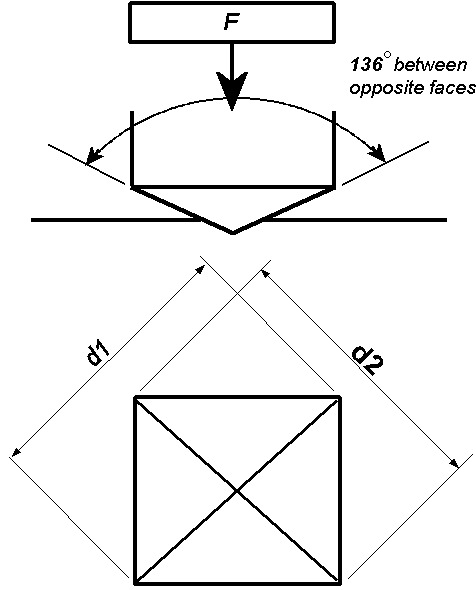
\includegraphics[width=0.8\textwidth]{figures/3537580_orig-0000.jpg}
            \caption{Diagram showing the diamond-shaped indenter with the 136° angle and diagonals \(d_1\) and \(d_2\).}
            \label{fig:vickers-diagram}
        \end{minipage}\hfill
        \begin{minipage}{0.51\textwidth}
            The Vickers hardness (\(HV\)) is calculated using the applied force (\(F\)) and the surface area (\(A\)) of the indentation. 
            \begin{equation}
                    HV = \frac{F}{A}
            \end{equation}
            \begin{itemize}[itemsep=-1mm]
                \item \(HV\): Vickers hardness (dimensionless)
                \item \(F\): Applied force (kgf or N)
                \item \(A\): Surface area of the indentation (mm\(^2\))
                
            \end{itemize}
            The formula for $A$ incorporates the geometry of the diamond pyramid indenter, 
            Such that surface area \(A\) can be expressed as:
            \begin{equation}
                A = \frac{d^2}{2\sin\left(\frac{136^\circ}{2}\right)}
            \end{equation}
            Where:  
            \begin{itemize}[itemsep=-1mm]
                \item \(A\): Surface area of the indentation (mm\(^2\))
                \item \(d\): Arithmetic mean of the diagonals \(d_1\) and \(d_2\) (mm)
            \end{itemize}
            in so that it is equivalent to:
            \begin{equation}
                    A= \frac{\left(\frac{d_1+d_2}{2}\right)^2}{2\sin\left(\frac{136^\circ}{2}\right)} \approx 0.1382\left(d_1 + d_2\right)^2
            \end{equation}
        \end{minipage}\\
    \end{figure}
    \vspace{-0.1em}\noindent
    The HV5 test, for instance, applies a fixed load of 5 kgf (49.03 N), and the hardness is calculated as:  
    \begin{equation}
        HV5 = \frac{49.03}{A} \approx \frac{354.78}{\left(d_1 + d_2\right)^2}
    \end{equation}
The test procedure involves measuring the two diagonals of the indentation under a microscope and squaring their sum. The resulting hardness value is expressed as a dimensionless number, such as \(HV30\), which denotes the hardness under a 30 kgf load.  

\subsubsection*{Importance and Applications}  

The Vickers hardness test is particularly useful for evaluating materials with fine microstructures or thin coatings, as it can accurately measure small indentations. The test’s precision and ability to quantify hardness provide critical information about a material’s resistance to deformation, making it invaluable for quality control and research in metallurgy, engineering, and materials science.  

\newpage
\subsection{BHN (Brinell Hardness Number)}
The Brinell Hardness Number (BHN) measures a material's resistance to deformation, determined by the indentation left by a hard steel or carbide ball pressed into the material under a specified load. This test is commonly used for materials with a coarse or heterogeneous grain structure.\\[1em]
The formula for calculating the Brinell Hardness Number is:
\begin{equation}
    BHN = \frac{2P}{\pi D (D - \sqrt{D^2 - d^2})}
\end{equation}
Where:
\begin{itemize}[itemsep=-1mm]
    \item \( P \) : applied load in kilogram-force (kgf),
    \item \( D \) : diameter of the indenter (typically 10 mm),
    \item \( d \) : diameter of the indentation (mm).
\end{itemize}
\textbf{Note}: The Brinell test may use either $P$ or $F$ for the load, depending on the source.\\ 
The BHN provides insight into a material's ability to resist wear and deformation, which is important for assessing the durability and suitability of metals in various engineering applications. BHN values are particularly useful for testing larger, rougher materials and are commonly applied to metals like steel and cast iron. The results help predict wear resistance and strength under load.

\end{document}
